\section{Die thermodynamischen Potentiale}

\subsection{Skalierung von Systemen}

Die positive Zahl $\lambda \in \R_{>0}$ sei der Skalierungsfaktor. Sei hier
$\lambda = 2$. Weiter sei $S \in \S$ ein System, welches wir skalieren, also
um den Faktor $\lambda = 2$ vergrössern möchten. Die Beschreibung des
skalierten Systemes, welches fortan $2S$ genannt wird, ist dann eine
"eingeschränkte Beschreibung" von $S \vee S'$, wobei $S' \cong S$ eine
Kopie von $S$ ist. Für $2S$ sollen nicht alle Zustände und Prozesse erlaubt
sein, die auf $S \vee S'$ möglich sind.
\begin{enumerate}[(i)]
    \item Die Zustände von $2S$ sind von der Form $\sigma \vee \sigma'$,
        wobei $\sigma \in \Sigma_S$ und $\sigma' \in \Sigma_{S'}$ der zu
        $\sigma$ äquivalente Zustand ist. D.h. der Zustandsraum ist
        $\Sigma_{2S} = \geschwungeneklammer{\sigma \vee \sigma' \ | \
        \sigma \in \Sigma_S , \ \sigma \cong \sigma' \in \Sigma_{S'}}$.
    \item Genauso sind die Prozesse auf $2S$ von der Form $p \vee p'$, wobei
        $p' \cong p$ der zu $p$ äquivalente Prozess ist. Insbesondere ist
        die Menge der Arbeitsprozesse auf $2S$ gleich $\P_{2S} =
        \geschwungeneklammer{p \vee p' \ | \ p \in \P_S , \ p \cong p' \in
        \P_{S'}}$.
\end{enumerate}
Ein allgemeiner Prozess auf $2S$ wird also den Zustandsraum $\Sigma_{2S}$
respektieren, d.h. er darf Zustände der Form $\sigma_1 \vee \sigma_1'$ nur
solche der Form $\sigma_2 \vee \sigma_2'$ überführen. Im Zusammenhang mit
skalierten Systemen schreiben wir ab jetzt $2\sigma := \sigma \vee \sigma'$
für Zustände auf $2S$. Gleiches foll für Arbeitsprozesse gelten,
$2p := p \vee p'$.

Äquivalent: Ein um den Faktor $\lambda \in \N$ skaliertes System vom System
$S$ ist $S^{(1)} \vee \dotsb \vee S^{(\lambda)}$ mit $S \cong S^{(i)} \ \forall
i =1,\dots,\lambda$. Falls $\lambda = \frac{1}{\nu}$ für ein $\nu \in \N$,
wird $\lambda \sigma$ definiert als der folgende Zustand:
\begin{align*}
    \underbrace{\lambda \sigma \vee \dotsb \vee \lambda \sigma}_{\nu \text{ mal}}
    = \sigma
\end{align*}
Für $\lambda = \frac{\mu}{\nu}$ definiert man $\lambda \sigma = \mu
\klammer{\frac{1}{\nu} \sigma}$. Da $\Q$ dicht ist in $\R$ folgt die
Aussage für beliebige $\lambda \in \R$.

\begin{definition}[Homogene Zustandsvariablen]
    Sei $S \in \S$ und $X_S$ eine Zustandsvariable von $S$, welche
    für beliebige $\lambda \in \R$ zugehörige Zustandsgrössen $X_{\lambda S}$
    auf den skalierten Systemen $\lambda S$ kennt. Eine solche Zustandsvariable
    heisst homogen vom Grad $k$ falls
    \begin{align*}
        X_{\lambda S} (\lambda \sigma) = \lambda^k X_{S} (\sigma)
    \end{align*}
    für alle $\sigma \in \Sigma_S$ und alle $\lambda \in \R$. Zustandsgrössen,
    die homogen vom Grad $0$ sind, heissen intensiv. Solche, die homogen
    vom Grad $1$ sind, heissen extensiv.
\end{definition}


\subsection{Das Extremalprinzip für die Entropie}

Betrachte ein zusammengesätztes System $S = S' \vee S''$, welches zunächst
in einem Zustand $\sigma' \vee \sigma''$ ist. Zunächst sind $S'$ und $S''$
nicht im thermischen Kontakt. Für die Entropie des Anfangszustands
$\sigma' \vee \sigma''$ gilt:
\begin{align*}
    S_S(\sigma' \vee \sigma'') = S_{S'} (\sigma) + S_{S''} (\sigma'')
\end{align*}
$\sigma' \vee \sigma''$ wird manchmal gehemmter Gleichgewichtszustand genannt.
Entfernen der Trennwand ist ein Arbeitsprozess auf $S$, wenn $S$ ansonsten
isoliert ist, der keine Arbeit kostet. Wir bezeichnen den Endzustand nach
Entfernen der Trennwand mit $\sigma' + \sigma''$. Der Endzustand wird als
vollständiges Gleichgewicht bezeichnet. Nach dem Entropiesatz gilt für
Arbeitsprozesse (insbesondere adiabatische Prozesse): $S_S (\sigma' \vee
\sigma'') \leq S_S (\sigma' + \sigma'')$ und Gleichheit falls das Entfernen
der Wand reversibel ist.

\begin{theorem}[Extremalprinzip der Entropie]
    Für $S \in \S$ und $\sigma \in \Sigma_S$ sowie jede mögliche disjunkte
    Aufteilung von $S$ in Subsysteme $S',S'' \in \S$ ($S = S' \vee S''$)
    gilt
    \begin{align*}
        S_S (\sigma) \max_{\stackrel{\sigma',\sigma''}{\sigma' + \sigma'' = \sigma}}
            S_{S'} (\sigma') + S_{S''}(\sigma'')
    \end{align*}
    wobei die Zustände $\sigma' \in \Sigma_{S'}$ und $\sigma'' \in \Sigma_{S''}$
    Zustände der Systeme $S'$ und $S''$ sein sollen. Informell heisst das,
    dass in einem abgeschlossenen System die Entropie maximal ist, wenn
    der Gesamtzustand im Gleichgewicht ist.
\end{theorem}

\subsection{Homogenität}

Für einen Arbeitsprozess, bei dem sowohl Substanzmenge als auch Volumen
verändert werden können, soll von nun an gelten, dass
\begin{align*}
    \delta W = - p dV + \mu d N
\end{align*}
Die neue Grösse $\mu$, die eine Zustandsgrösse ist, heisst chemisches Potential.
Wir können weiter herleiten:

\begin{align*}
    dS = \frac{1}{T} \klammer{dU + p dV - \mu dN}
\end{align*}
Daraus folgt:
\begin{align*}
    \frac{\partial S}{\partial U} \Big|_{V,N} = \frac{1}{T}
    \hspace{15pt} , \hspace{15pt}
    \frac{\partial S}{\partial V} \Big|_{U,N} = \frac{p}{T}
    \hspace{15pt} , \hspace{15pt}
    \frac{\partial S}{\partial N} \Big|_{U,V} = - \frac{\mu}{T}
\end{align*}

\paragraph{Homogenitätsrelation}
\begin{align*}
    S = U \frac{\partial S}{\partial U} \Big|_{V,N} +
        V \frac{\partial S}{\partial V} \Big|_{U,N} +
        N \frac{\partial S}{\partial N} \Big|_{U,V}
    = \frac{1}{T} \klammer{U + p V - \mu N}
\end{align*}


\subsection{Konkavität der Entropie}

Betrachte $\alpha',\alpha'' \in \R$ mit $\alpha' + \alpha'' = 1$. Seien
$\sigma' \in \Sigma_{S'}$ und $\sigma'' \in \Sigma_{S''}$ Zustände auf $S'$
respektive $S''$ und damit $\alpha' \sigma' \in \Sigma_{\alpha' S'}$ und
$\alpha'' \sigma'' \in \Sigma_{\alpha'' S''}$ wieder Zustände auf $\alpha' S'$
respektive $\alpha'' S''$. Dann gilt gemäss dem Extremalprinzip und der
Extensivität der Entropie, dass
\begin{align*}
    S(\alpha' \sigma' + \alpha'' \sigma'') \geq
    \alpha' S(\sigma') + \alpha'' S(\sigma'')
\end{align*}

\begin{theorem}[Äquivalenz von Eigenschaften der Entropie]
    Folgende Aussagen sind äquivalent:
    \begin{enumerate}[(i)]
        \item $S(\sigma)$ ist linear zwischen $\sigma'$ und $\sigma''$.
        \item $S(\sigma' + \sigma'') = S(\sigma') + S(\sigma'')$, d.h.
            $\sigma'$ und $\sigma''$ sind im vollständigen Gleichgewicht.
        \item $\mathbf{\nabla} S(\sigma') = \mathbf{\nabla} S(\sigma'')$, d.h
            für $\sigma = (U,V,N)$ gilt $T' = T''$, $p' = p''$ und $\mu' = \mu''$.
            Hier ist:
            \begin{align*}
                \mathbf{\nabla} S(\sigma) = \begin{pmatrix}
                    \frac{\partial S}{\partial U} \Big|_{V,N} &
                    \frac{\partial S}{\partial V} \Big|_{U,N} &
                    \frac{\partial S}{\partial N} \Big|_{U,V}
                \end{pmatrix}
            \end{align*}
    \end{enumerate}
\end{theorem}

\begin{theorem}[Gibbs-Duhem Relation]
    Es gilt:
    \begin{align*}
        S dT - V dp + N d \mu = 0
    \end{align*}
    Insbesondere sind nur zwei der drei Zustandsgrössen $T,p$ und $\mu$
    unabhängig.
\end{theorem}

\subsection{Stabilitätsbedingungen}

Konkavität der Entropie ist gleichbedeutend damit, dass die Hesse-Matrix
\begin{align*}
    \partial^2 S = \begin{pmatrix}
        \frac{\partial^2 S}{\partial U^2} &
        \frac{\partial^2 S}{\partial U \partial V} \\
        \frac{\partial^2 S}{\partial V \partial U} &
        \frac{\partial^2 S}{\partial V^2}
    \end{pmatrix}
\end{align*}
in jedem Punkt $(U,V,N=1)$ negativ semidefinit ist. Insbesondere:
\begin{align*}
    \frac{\partial^2 S}{\partial U^2} \leq 0
    \hspace{10pt} , \hspace{10pt}
    \det (\partial^2 S) \geq 0
\end{align*}

\begin{definition}[Wärmekapazität und Kompressibilität]
    Die spezifische Wärme für festes Volumen $V$ und diejenige für
    festen Druck $p$ sind:
    \begin{align*}
        C_V :=& \frac{\delta Q}{\partial T} \Big|_{V}
        = \frac{\partial U}{\partial T} \Big|_{V}
        \\
        C_p :=& \frac{\delta Q}{\partial T} \Big|_{p}
            = T \frac{\partial S}{\partial T} \Big|_{p}
            = \frac{\partial U + p \partial V}{\partial T} \Big|_{p}
            = \frac{\partial U}{\partial T} \Big|_{p} + p \frac{\partial V}{\partial T} \Big|_{p}
    \end{align*}
    Die isotherme Kompressibilität ist definiert als
    \begin{align*}
        \kappa_T := - \frac{1}{V} \frac{\partial V}{\partial p} \Big|_{T}
    \end{align*}
    Es gilt $C_V \geq 0, \kappa_T \geq 0$ und $C_p \geq 0$. Weiter gilt:
    \begin{align*}
        C_p - C_V = \frac{T V \alpha^2}{\kappa_T} \geq 0
    \end{align*}
    mit $\alpha = \frac{1}{V} \frac{\partial V}{\partial T} \Big|_p$.
\end{definition}


\subsection{Weitere thermodynamischen Potentiale}

\subsubsection{Die Legendre Transformation}

\begin{definition}[Legendretransformierte]
    Sei $D \subset \R^n$ und $f: D \rightarrow \R$. Die Legendretransformierte
    $f^\ast$ von $f$ ist definiert für jene $p \in \R^n$, für welche
    \begin{align*}
        f^\ast (p) = \sup_{x \in D} \klammer{ p \cdot x - f(x)}
    \end{align*}
    endlich ist. Wir nennen den Definitionsbereich $D^\ast$.
\end{definition}

\begin{theorem}
    Sei $f: D \rightarrow \R$ eine reelle Funktion. Dann gilt:
    \begin{enumerate}[(i)]
        \item $f^\ast : D^\ast \rightarrow \R$ ist konvex.
        \item Ist $f$ konvex, so ist $f^{\ast \ast} = f$ (mit $D^{\ast \ast} = D)$
        \item Ist $f=f(x,y)$ konvex in $(x,y)$, so ist $f^\ast (p,y)$ konkav in $y$.
            \begin{align*}
                f^\ast (p,y) = \sup_x \eckigeklammer{p \cdot x - f(x,y)}
            \end{align*}
    \end{enumerate}
    Ist $f(S,V,N)$ konvex, so ist $f^{\ast(S \rightarrow T)} (T,V,N)$ konvex in
    $T$ und konkav in allen anderen Variablen.
\end{theorem}

\begin{bemerkung}
    Ist $f$ differenzierbar und konvex, so gelten
    \begin{align*}
        \klammer{f^\ast}'(p_0) = x_0
        \hspace{10pt} , \hspace{10pt}
        \klammer{f^\ast}' = \klammer{f'}^{-1}
    \end{align*}
    Falls $f$ strikt konvex und differenzierbar ist, gilt sogar
    \begin{align*}
        x_0 = \klammer{f'}^{-1} (p_0)
    \end{align*}
\end{bemerkung}

\subsubsection{Energie}

Homogenitätsrelation: $U = T S - p V + \mu N$. $U(S,V,N)$ ist konvex in $S,V$
und $N$. Insbesondere gilt:
\begin{align*}
    dU = T dS - p dV + \mu dN
\end{align*}
Daraus folgt:
\begin{align*}
    \frac{\partial U}{\partial S} \Big|_{V,N} = T
    \hspace{10pt} , \hspace{10pt}
    \frac{\partial U}{\partial V} \Big|_{S,N} = -p
    \hspace{10pt} , \hspace{10pt}
    \frac{\partial U}{\partial N} \Big|_{S,V} = \mu
\end{align*}

\subsubsection{Die (Helmholtz) freie Energie}
\begin{align*}
    F(T,V,N) = U(S,V,N) - T S = - p V + \mu N
\end{align*}
wobei $S$ als Lösung von $\frac{\partial U}{\partial S} \Big|_{V,N} = T$
aufgefasst wird. $F$ ist homogen vom Grad $1$ in $V$ und $N$. Weiter folgt:
\begin{align*}
    dF = dU - T dS - S dT
    = -p dV + \mu dN - S dT
\end{align*}
Daraus folgt:
\begin{align*}
    \frac{\partial F}{\partial T} \Big|_{V,N} = -S
    \hspace{10pt} , \hspace{10pt}
    \frac{\partial F}{\partial V} \Big|_{T,N} = -p
    \hspace{10pt} , \hspace{10pt}
    \frac{\partial F}{\partial N} \Big|_{T,V} = \mu
\end{align*}
$F(T,V,N)$ ist konkav in $T$ und konvex in $(V,N)$.

\paragraph{Extremalprinzip für Helmholtz freie Energie}
Bei fixem Gesamtvolumen, fixer Gesamtstoffmenge und fixer Temperatur ist $F$
im Gleichgewicht minimal.

\paragraph{Maxwell-Relationen}
Folgen aus $\frac{\partial^2 F}{\partial T \partial V} =
\frac{\partial^2 F}{\partial V \partial T}$ und anderen partiellen
Ableitungen.
\begin{align*}
    \frac{\partial S}{\partial V} \Big|_{T,N}
    = \frac{\partial p}{\partial T} \Big|_{V,N}
    \hspace{5pt} , \hspace{5pt}
    - \frac{\partial p}{\partial N} \Big|_{T,V}
    = \frac{\partial \mu}{\partial V} \Big|_{T,N}
    \hspace{5pt} , \hspace{5pt}
    - \frac{\partial S}{\partial N} \Big|_{T,V}
    = \frac{\partial \mu}{\partial T} \Big|_{V,N}
\end{align*}

\subsubsection{Die Enthalpie}
\begin{align*}
    H(S,p,N) = U(S,V,N) + p V = T S + \mu N
\end{align*}
wobei $V$ eine Lösung von $\frac{\partial U}{\partial V} \Big|_{S,N} = -p$ ist.
Weiter folgt:
\begin{align*}
    dH = dU + p dV + V dp = T dS + V dp + \mu dN
\end{align*}

\subsubsection{Die Gibbs'sche freie Energie}
\begin{align*}
    G(T,p,N) &= U(T,p,N) - T S(T,p,N) + p V(T,p,N)
    \\
    &= F(T,p,N) + p V(T,p,N) = H(T,p,N) - T S
    \\
    &= \mu(T,p) N 
    \\
    dG &= dU - d(TS) + d(pV) = -S dT + V dp + \mu dN
\end{align*}

\subsubsection{Das Grosskanonische Potential}
\begin{align*}
    \Omega(T,V,\mu) &= U(S,V,N) - T S - \mu N
    = F(T,V,N) - \mu N
    = -p(T,\mu) V
    \\
    d \Omega &= - S dT - p dV - N d \mu
\end{align*}

\subsection{Konkavität, Konvexität und Extremalprinzip}

Die freie Energie $F(T,V,N)$ ist konkav in $T>0$ und konvex in $(V,N)$.
Die Enthalpie $H(S,p,N)$ ist konkav in $p$ und konvex in $(S,N)$.
Die Gibbs'sche freie Energie $G(T,p,N)$ ist konkav in $(T,p)$ und linear in $N$.
Das Grosskanonische Potential $\Omega(T,V,\mu)$ ist konkav in $(T,\mu)$ und
linear in $V$.

\paragraph{Extremalprinzip der freien Energie}
"Bei bestem Gesamtvolumen und fester Temperatur ist die freie Energie im
vollständigen Gleichgewicht minimal."
\begin{align*}
    F(T,V',N') + F(T,V'',N'') \geq F(T,V' + V'' , N' + N'')
\end{align*}


\subsection{Reine und gemischte Phasen}

Angenommen jeder Zustand $\sigma = (U,V)$ zu einem $(T,p)$ ist eindeutig
darstellbar als "Mischung" $\sigma = \sum_{i}^N \alpha_i \sigma_i$ mit $\alpha_i
\geq 0 \ \forall i$ und $\sum_{i}^N \alpha_i = 1$ wobei $N=1,2,3$.

Die Extremalpunkte der konvexen Berührungsfigur (hier $\sigma_1,\sigma_2,
\sigma_3$) heissen reine Phasen. Diese Punkte sind definiert als diejenigen
Zustände, die nicht innerhalb der Verbindungsstrecke von zwei anderen Punkten
liegen und man somit nicht als echte Mischung von zwei Zuständen zum selben
$(T,p)$ auffassen kann.

\paragraph{Gibbs'sche Phasenregel}

Die Gibbs'sche Phasenregel besagt, dass die Berührungsflächen
Simplices\footnote{Ein Simplex ist ein $n$-dimensionales Polytop mit
$n+1$ Ecken (Extremalpunkte). Dies ist die kleinste Anzahl Ecken, die
ein $n$-dimensionales Polytop haben kann.} sind. Sei nun $n$ die Anzahl
koexistierender Phasen in einer Mischung und $f$ die Anzahl freier intensiver
Grössen bei festem $n$. Dann besagt die Gibbs'sche Phasenregel ferner, dass
Simplizes in Scharen vorkommen: Für ein System mit zwei Koordinaten $(U,V)$
ist
\begin{align*}
    f = 3 - n
\end{align*}

\begin{figure}[h]
    \centering
    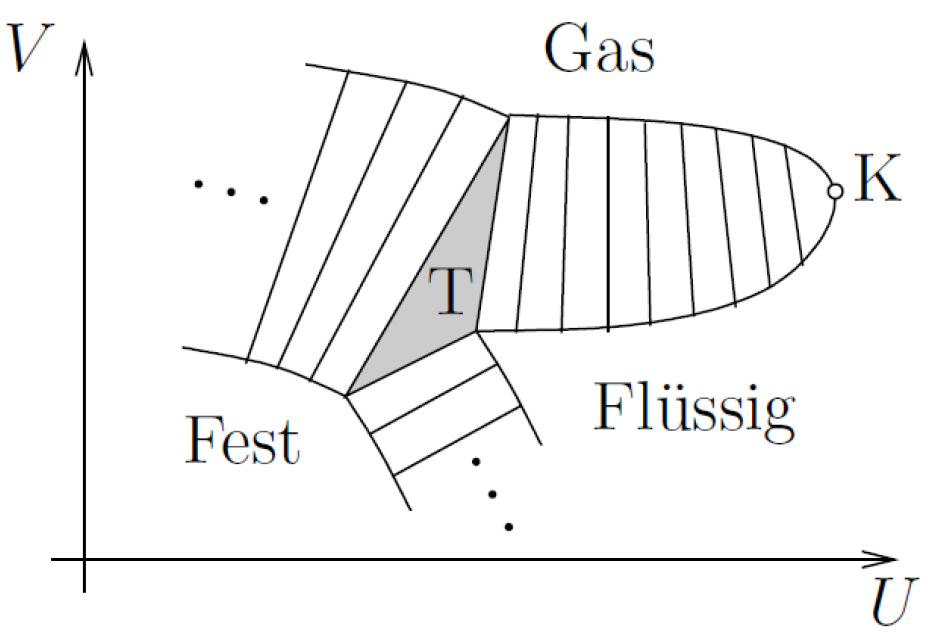
\includegraphics[width=0.25\textwidth]{Bilder/Gibbs_UV.png}
    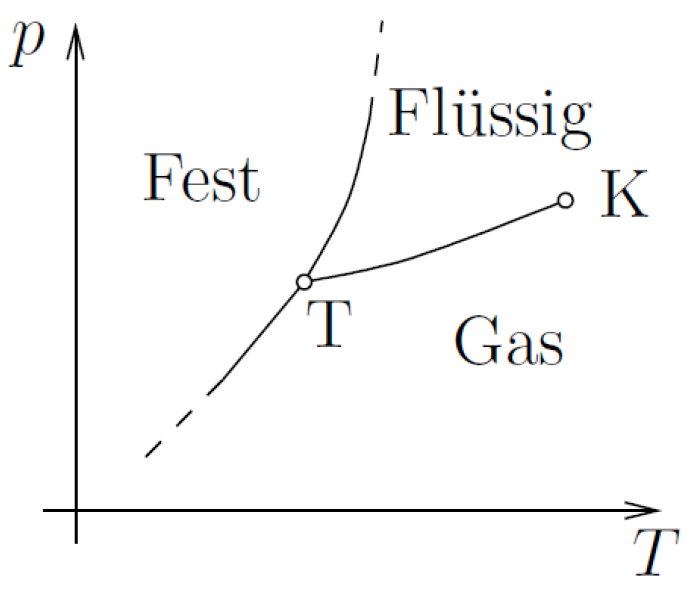
\includegraphics[width=0.2\textwidth]{Bilder/Gibbs_Tp.png}
    \caption{Links: Entropiefläche (Ansicht von oben) im $U-V$ Diagramm.
        Rechts: Das zugehörige $p-T$ Phasendiagramm.}
    \label{Gibbs}
\end{figure}

Die weissen Gebiete im $U-V$ und im $p-T$ Diagramm entsprechen reinen Phasen:
Die Entropie ist dort strikt konkav und der Zusammenhang $(U,V) \leftrightarrow
(T,p)$ bijektiv. Bei einem Phasenübergang $n$-ter Ordnung ist $G$ als Funktion
von $T$ und $p$ in seinen ersten $n-1$ Ableitungen stetig, die $n$-te
Ableitung ist stetig. Ein erster Ordnung Phasenübergang involviert generell
latente Wärme, d.h. es wird Energie vom System aufgenommen oder abgegeben,
ohne dass dies eine Temperaturänderung zur Folge hat.

\paragraph{Gleichung von Claisius-Clapeyron}
\begin{align*}
    \frac{\partial p}{\partial T} \equiv
    \frac{\partial p}{\partial T} \Big|_{V,N}
    = \frac{\partial S}{\partial V} \Big|_{T,N}
    = \frac{S_2 - S_1}{V_2 - V_1}
    = \frac{L_{12}}{T (V_2 - V_1)}
\end{align*}
Da $\frac{\partial p}{\partial T}$ unabhängig ist von $V$, muss auch
$\frac{\partial S}{\partial V} \Big|_{T,N}$ unabhängig von $V$ sein. Also ist
$S$ linear in $V$. $L_{12}$ ist die Übergangswärme von Phase 1 zu Phase 2.
Es gilt:
\begin{align*}
    L_{12} := \int_{\sigma_1}^{\sigma_2} \delta Q
    = \int_{\sigma_1}^{\sigma_2} T dS = T (S_2 - S_1)
\end{align*}
Für ein Wasser-Eis Gemisch ist $L_{12} > 0$, aber $V_2 - V_1 < 0$ und
somit $\frac{\partial p}{\partial T} < 0$. Also kann bei isothermer
Druckzunahme Eis schmelzen.

